\chapter{Beobachter}
\section{Zielsetzung}
\begin{itemize}
    \item Warum wird ein Beobachter benötigt?
    \item Entwicklung eines Beobachters zur Schätzung von Zuständen, die nicht direkt messbar sind.
    \item Welche Zuständer werden nicht gemessen?
\end{itemize}
\section{Beobachtermodell}
\subsection{Kinematisches Modell}
\begin{itemize}
    \item Inverse Kinematik von \ref{eq:Koordinatentransformation} => Umrechnung Roboterkoordinaten
    \item Umrechnung in Weltkoordinaten (wichtig, dass es zyclisch abläuft, da winkeländerung zu änderung in x/y berechnung führt)
    \item Resultat: Aus Motordaten und Anfangsposition kannn die aktuelle Position im Raum berechnet werden
\end{itemize}
\subsection{Beobachterstrucktur}
\begin{itemize}
    \item Luneburger
    \item EKF
    \item Zu beiden Blockschaltbilder erstellen
    \item Vergleichen und aufzeigen, warum EKF keinen bedeutenden Vorteil gegenüber Luneburger hat (Kamerafehler ist immer ähnlich, daher reicht statischer Gain)
\end{itemize}
\section{Parametrierung}
\begin{itemize}
    \item Einstellen des Gains L
    \item Variabler Gain
\end{itemize}
\begin{figure}[H]
    \centering
    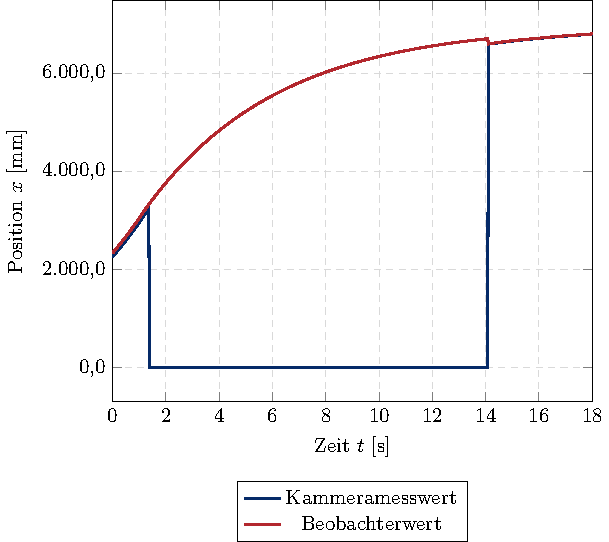
\includegraphics[width=0.8\textwidth]{_Grafiken/Obs_L1_Gesammt.pdf}
    \caption{Beobachter mit direktem Ausgleich Gesammt}
    \label{fig:Obs_L1_Gesammt}
\end{figure}
\begin{figure}[H]
    \centering
    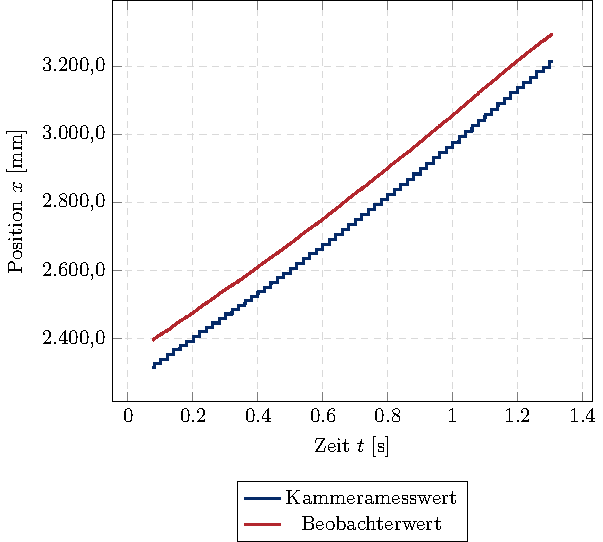
\includegraphics[width=0.8\textwidth]{_Grafiken/Obs_L1_Normalfahrt.pdf}
    \caption{Beobachter mit direktem Ausgleich Normalfahrt}
    \label{fig:Obs_L1_Normalfahrt}
\end{figure}
\begin{figure}[H]
    \centering
    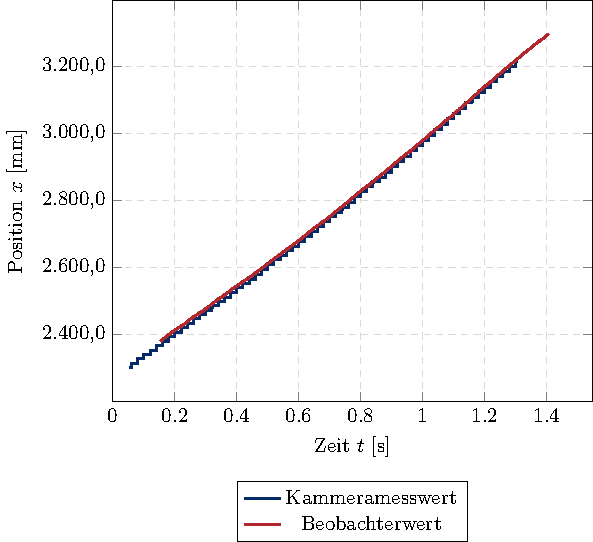
\includegraphics[width=0.8\textwidth]{_Grafiken/Obs_L1_NormalfahrtVerschoben.pdf}
    \caption{Beobachter mit direktem Ausgleich Normalfahrt Verschoben}
    \label{fig:Obs_L1_NormalfahrtVerschoben}
\end{figure}
\begin{figure}[H]
    \centering
    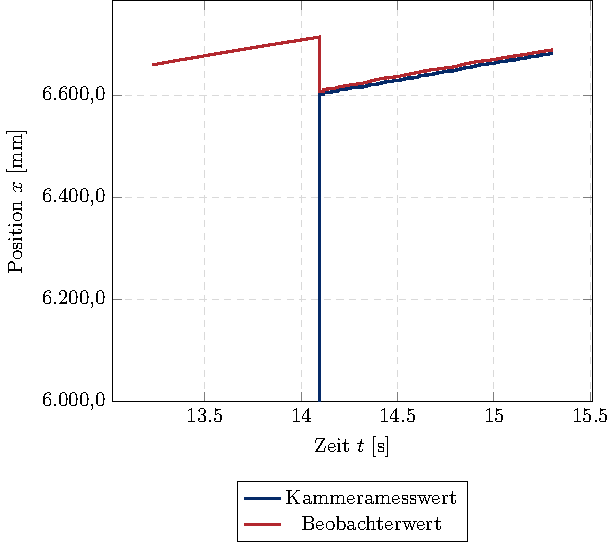
\includegraphics[width=0.8\textwidth]{_Grafiken/Obs_L1_Ausgleich.pdf}
    \caption{Beobachter mit direktem Ausgleich}
    \label{fig:Obs_L1_Ausgleich}
\end{figure}

\begin{figure}[H]
    \centering
    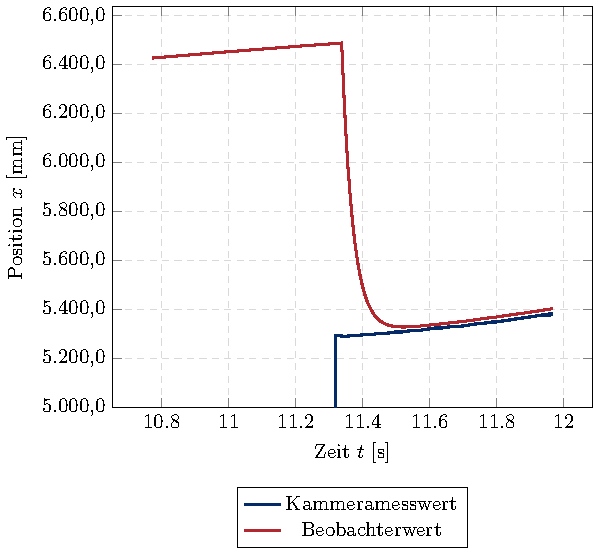
\includegraphics[width=0.8\textwidth]{_Grafiken/Obs_L01_Ausgleich.pdf}
    \caption{Beobachter mit langsamen Ausgleich}
    \label{fig:Obs_L01_Ausgleich}
\end{figure}

\begin{figure}[H]
    \centering
    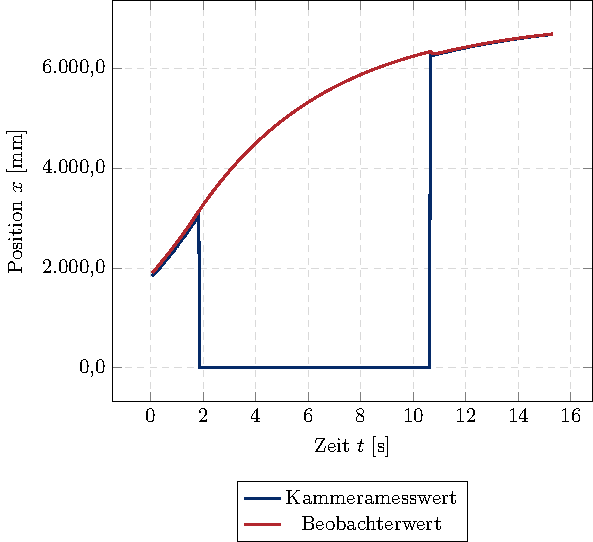
\includegraphics[width=0.8\textwidth]{_Grafiken/Obs_VarGain_Gesammt.pdf}
    \caption{Beobachter mit variablen Gain}
    \label{fig:Obs_VarGain_Gesammt}
\end{figure}
Is von der Idee her ganz nett, aber kein großer Effekt, da die Kamera, wenn Bild Erkannt, immer ähnlichen Fehler aufweißt. Also lieber statischen Wert tunen.